Ein weiterer Teil der Aufgabe befasst sich mit dem Greifen der Tasse. Daf�r steht der Greifer Schunk PG70 zur Verf�gung, sowie ein 3D-Drucker zur Erstellung von Fingern. Zu Beginn wurden zwei Griffvarianten diskutiert: 1) Seitliches Greifen und 2) Greifen von oben. W�hrend seitliches Greifen nat�rlicher erscheint, erwies sich die Planung f�r einen Griff der Tasse von oben als einfacher. Um einen vorzeitigen Ausschluss der Variante zu vermeiden, wurde ein Fingermodell mit zwei m�glichen Grifffl�chen erstellt, eine Fl�che am Ende des Fingers, sowie eine Ausbuchtung am Schaft des Fingers. Die Fl�che am Endes des Fingers f�hrte zu genau zwei Kontaktpunkten zwischen der Tasse und dem Endeffektor. Die Tasse wurde sehr instabil gehalten und neigte zu Schaukeln bei schnellen Bewegung. Desweiteren reichte die Reibung zwischen Kunststoff und Ton nicht f�r einen festen Griff aus.

Aus diesem Grund wurden die Anzahl der Kontaktpunkte durch eine eckige Ausbuchtung von zwei auf vier verdoppelt. Bei ersten Tests mit der eigentlichen Hardware wurde ein weiteres Problem erkannt: Der Gesamthub des Greifers ist geringer als der durchschnittliche Durchmesser einer Tasse. Daher konnte zuerst nur eine von zwei Tassen gegriffen werden, au�erdem beschr�nkte sich die Pufferzone auf weniger als 1cm pro Fingerbacke. Die ersten Ergebnisse aus der Bilderkennung legte eine deutliche Verbreitung der Griffbreite nahe, um Ungenauigkeiten bei der Approximation der Tasse auszugleichen. 

Die n�chste Generation an Fingern vergr��erte die Griffbreite um 4cm, erreicht durch "Nach-hinten"-Lagerung jeder Backe. Zus�tzlich wurde der Schaft verl�ngert und erhielt eine �hnliche kantige Ausbuchtung, wie bereits das Ende des Fingers. Diese �nderung vergr��erte den Arbeitsbereich des Roboters, den Sicherheitsabstand zum Tisch und die Kontaktfl�che der Tasse am Schaft. 

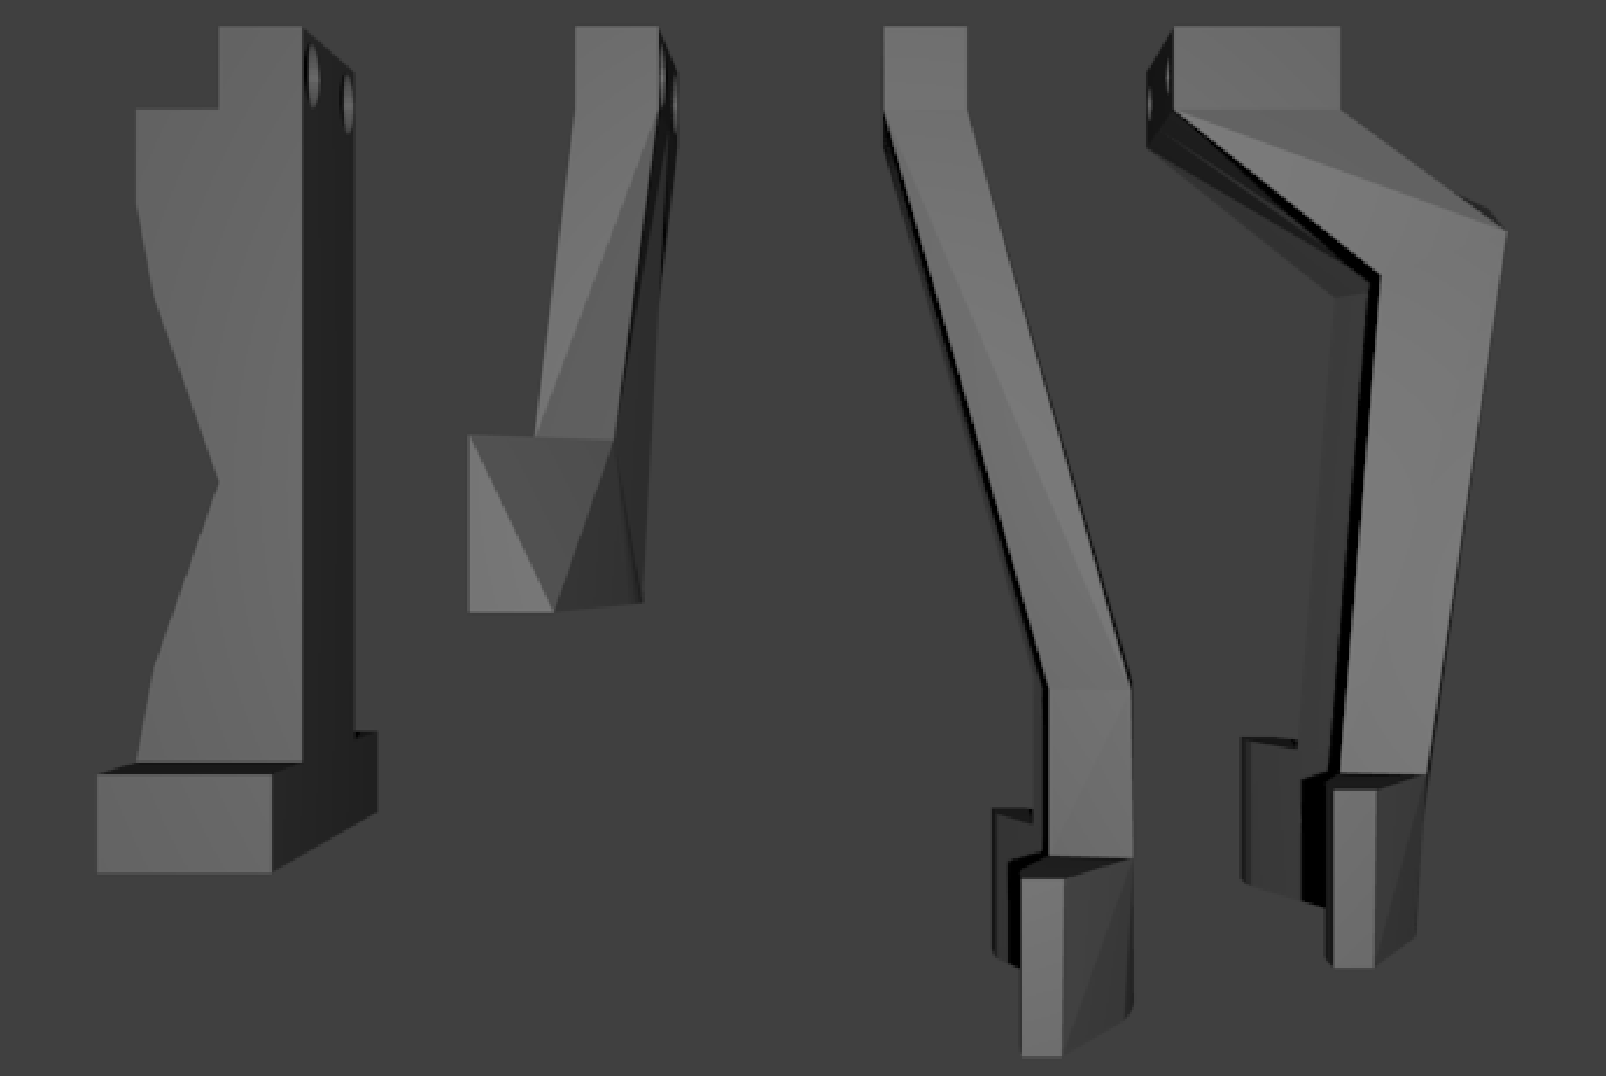
\includegraphics[width=\textwidth]{finger_evolution}

Bei weiteren Versuchen wurde durch einen Konfigurationsfehler zu tief unter die Kante der Tasse eingetaucht, was in letzter Konsequenz zum Brechen eines Fingers f�hrte. Um dieses Problem bei einer weiteren Iteration kategorisch auszuschlie�en, wurde die Verschiebung des Schaftes an den Montagebereich gelegt, eine abfallende Kante in Richtung Ende des Fingers konstruiert und die Gesamtl�nger von 12cm auf 11cm reduziert. F�r eine erh�hte Stabilit�t wurde die Druckrichtung von Horizontal auf Vertikal ver�ndert. 

Zus�tzlich wurden zwei Varianten f�r eine bessere Reibung getestet: 1) Arbeitshandschuh und 2) Haushaltsgummi. Aus dem Handschuh wurden zwei Finger entfernt und mit doppelseitigem Klebeband auf dem gedruckten Finger befestigt. Der Grip zwischen Finger und Tasse erh�ht sich, jedoch ist die hinzugef�gte Schicht d�nn, weshalb bei erh�htem Druck der Finger sich verbiegt. Zur Vermeidung wird eine dickere Schicht zwischen Finger und Tasse ben�tigt. Haushaltsgummis in einem X-Muster erweis sich als besser geeignet, da sie mehr Reibung und eine dickere Schicht bieten. 

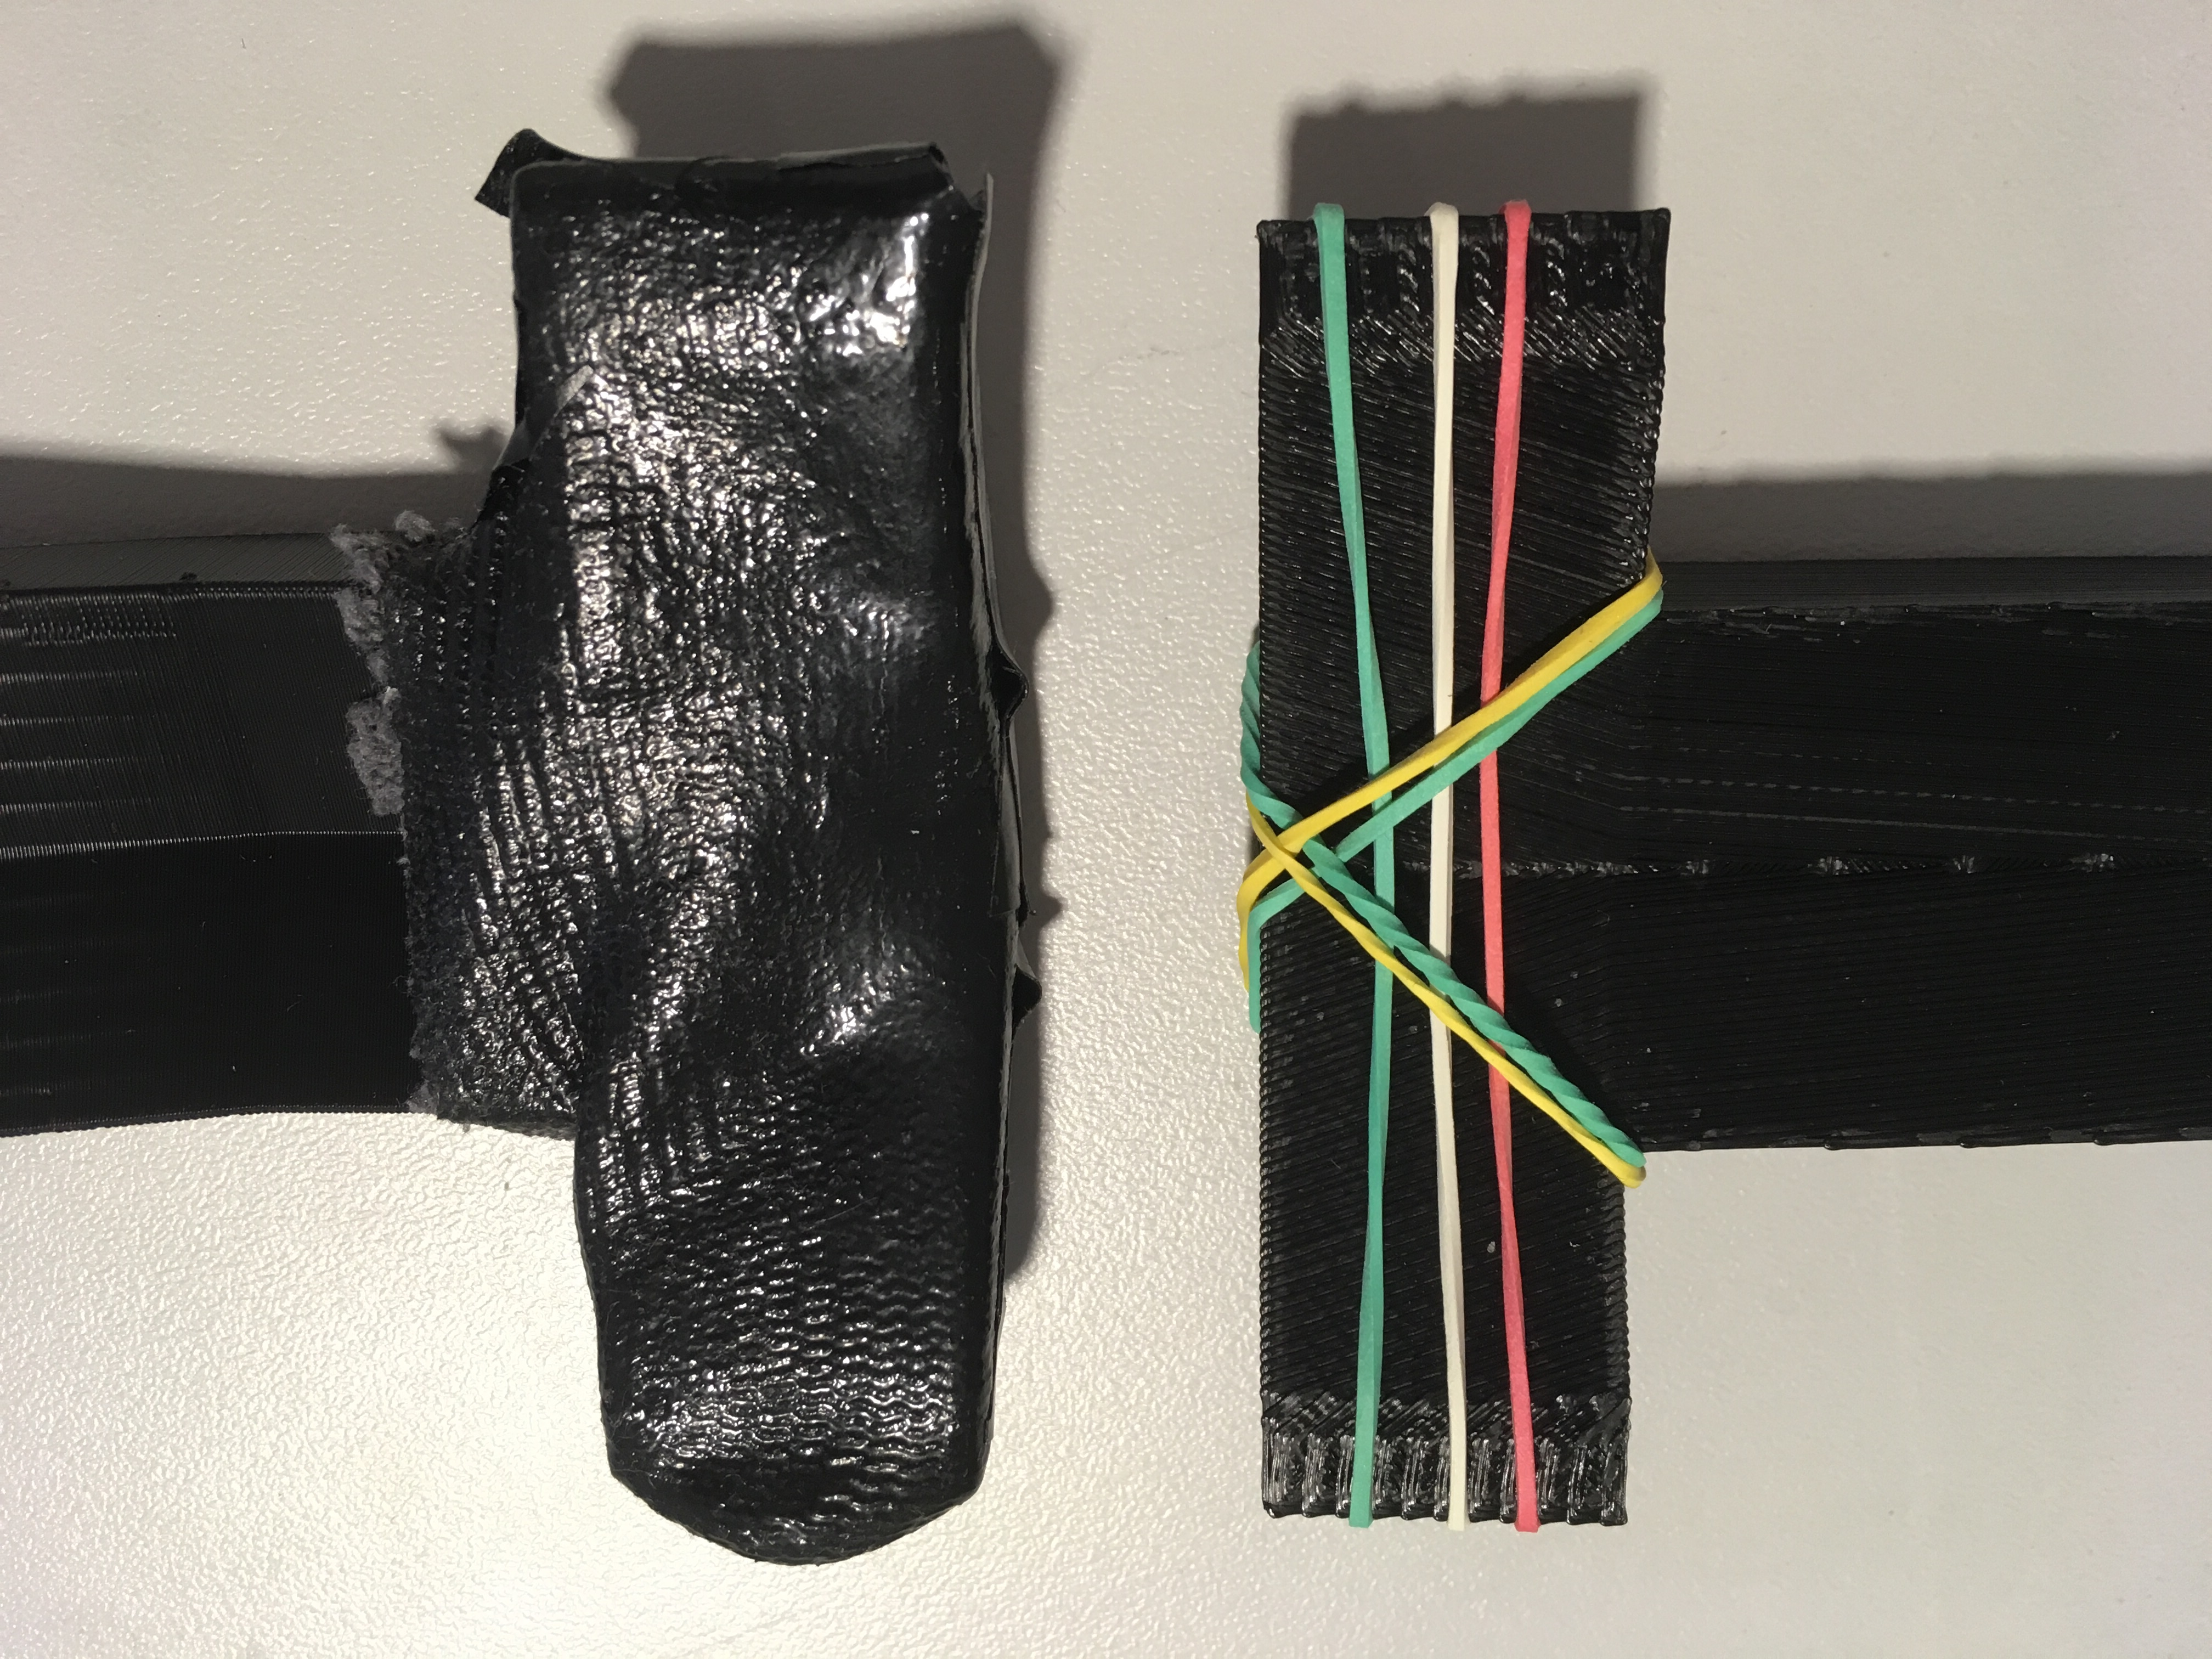
\includegraphics[width=\textwidth]{finger_tip}

Abh�ngig von der Tasse wurden verschiedene Konstanten f�r die Breite der Finger empirisch getestet. Zur Vereinfachung gehen wir nun von genau einem Tassenmodell mit einer festen Breite aus. Anfangs wurde mit einem Fingerabstand von 9mm gegriffen, jedoch l�sst sich dieser Wert zugunsten der Grifffestigkeit deutlich verkleinern. Es zeigte sich, dass bereits ein Abstand von 8mm ausreicht.

Nebenl�ufig zur Evolution der Finger wurde ein ROS Paket mit dem Namen "cup_gripper" erstellt. Die erste Variante beinhaltete zwei Services: GrabCup und ReleaseCup. GrabCup akzeptiert als Parameter cup_diameter in Meter und gibt, wie auch ReleaseCup, ein boolean success zur�ck. Es stellte sich heraus, dass Actions besser geeignet sind, da sie l�ngere Operation abbilden und Feedback geben k�nnen. Aus diesem Grund wurden die Services in Actions umgewandelt.
